\documentclass[12pt]{article}
\usepackage[utf8]{inputenc}

% Importing settings from setup.sty
\usepackage{setup}
\usepackage{booktabs}
\usepackage{multicol}
\usepackage{multirow}
\usepackage{glossaries}
% \makenoidxglossaries

% Acronyms
\newacronym{stt}{STT}{Speech-To-Text}
\newacronym{rnn}{RNN}{Recurrent Neural Network}
\newacronym{hmm}{HMM}{Hidden Markov Model}
\newacronym{lstm}{LSTM}{Long Short-Term Memory}
\newacronym{wer}{WER}{Word Rate Error}
\newacronym{swb}{SWB}{Switchboard}
\newacronym{fsh}{FSH}{Fisher}

% \pagenumbering{roman}
\begin{document}

% Inserting title page
\import{./}{title}

\pagenumbering{gobble}
\tableofcontents
% \listoffigures
% \listoftables

\newgeometry{
    left=25mm,
    right=25mm,
    top=25mm,
    bottom=25mm}
\pagenumbering{arabic}




%\setlength{\droptitle}{-5em}

% \title{\huge\textsc{Speech Recognition}}
% \author{UFUK CEM BIRBIRI \hspace{.5cm} JORIS LIMONIER }
% \date{\today}

\newpage
\pagenumbering{arabic}



\section{Introduction}
\subsection{Objective}
The objective of this project is to gain both a quantitative and a qualitative understanding of pre-trained voice recognition technologies. In particular, the first objective is to implement a \gls{stt} model using the DeepSpeech \cite{deepspeech_paper} library and evaluate the complexity of its deployment.

\subsection{The DeepSpeech Model}
Most of the traditional speech recognition systems use many engineered processing stages such as using specialized inputs, acoustic models or \gls{hmm} \cite{acoustic_model,hmm}. To improve the performance of these models, domain experts must exert huge effort to tune the features and models. With the help of deep learning algorithms, the performance of the speech recognition models has improved significantly \cite{dl1,dl2,dl3,dl4}.


The main idea of the DeepSpeech model \cite{deepspeech_paper} consist of \gls{rnn} trained on speech spectrograms and output English text transcriptions. In training phase multiple GPUs and and thousands of hours of data are used to create an end-to-end speech recognition system. The model has 5 hidden layers and is simpler than others models in the literature \cite{other_model1}. \gls{lstm} circuits are not used since they need computing and storing multiple gating neuron responses at each step. A drop-out rate between 5\% - 10\% was applied to only feed-forward layers and not to the recurrent hidden activations for regularization. It performs better than the previously proposed methods on the Switchboard Hub5'00 corpus where these traditional methods tend to give poor results in noisy environment. There is no need for hand-designed components for modelling background noise, variation of speakers or reverberation or noise filtering. Instead the model learns from a function which is robust to these effects. The evaluation of the results are done by \gls{wer}.

DeepSpeech achieves 16.0\% error on the full Switchboard Hub5'00 test set (LDC 2002S23), and outperforms the  commercial systems in noisy voice recognition tests. The authors reported that most of the errors occur because of the words that never or rarely appear in the train data.

The DeepSpeech model is trained on only the 300 hour Switchboard conversational telephone call data and trained on both \gls{swb} and \gls{fsh} \cite{data_cite}, a 2000 hour corpus that is collected in a similar manner as Switchboard. The testing is done on Switchboard Hub5'00 test set.

The authors propose two networks: DeepSpeech \gls{swb} and DeepSpeech \gls{swb} + \gls{fsh}. The DeepSpeech \gls{swb} model is a network of 5 hidden layers each with 2048 neurons trained on only 300 hour switchboard. The DeepSpeech \gls{swb} + \gls{fsh} model is an ensemble of 4 \glspl{rnn} each with 5 hidden layers of 2304 neurons trained on the full 2300 hour combined corpus.



\subsection{The Word Error Rate}
\label{wer_section}
\glspl{wer} is the most common evaluation metric in speech recognition tasks. It is calculated as:
\begin{equation*}
    \text{Word Error Rate} = \frac{\text{Substitutions + Insertions + Deletions}}{\text{Number of Words Spoken}}
\end{equation*}

\begin{enumerate}
    \item \textbf{Substitutions} occur when a word gets replaced (for example, “peach” is transcribed as “beach”)
    \item \textbf{Insertions} occur when a word gets added that was not said (for example, “watercolor” becomes “what are column”)
    \item \textbf{Deletions} are anytime a word is omitted from the transcript (for example, “how are you doing” becomes “how you doing”)
\end{enumerate}

\section{Problem solution}
\subsection{Our implementation of the model}
Our implementation of the model was run on Intel(R) Core(TM) i7-4710HQ CPU @ 2.50GHz laptop. \\
% /!\ This part is commented until we find the link to the dataset, in order not to forget to fill it
The dataset that we use can be found here:
\begin{verbatim}
https://isip.piconepress.com/projects/switchboard/
https://isip.piconepress.com/projects/switchboard/releases/
switchboard_icsi_ws97.tar.gz
\end{verbatim}
The project code can be found here:
\begin{verbatim}
https://github.com/jorislimonier/speech-recognition
\end{verbatim}
The steps that we made to get the predicted text output is as follows:
\begin{enumerate}
    \item Install DeepSpeech and pre-trained models
    \item Handle the RIFF id error by converting original wav files to a tmp wav file (expalined in \ref{riff error}).
    \item Perform \gls{stt} with DeepSpeech
    \item Evaluate the error rate using \gls{wer}.
\end{enumerate}

\subsection{The RIFF ID Error and How To Handle It}
\label{riff error}
An error occurred when trying to perform \gls{stt} with DeepSpeech. The error message was: \textit{ ``Failed to open file FILE.wav as a WAV due to: file does not start with RIFF ID."} After some research, it appears that this is due to having a 64-bit RIFF and that WAV does not support 64-bit RIFF files. To overcome this problem we read the WAV file with another library (librosa), write it back to a  WAV file (with soundfile), and then process it with DeepSpeech. These steps are displayed in the following piece of code:
\begin{verbatim}
import librosa
import soundfile as sf
x, _ = librosa.load(waf_file, sr=16000)
sf.write('tmp.wav', x, 16000)
wave.open('tmp.wav','r')
\end{verbatim}

\section{Results}
\label{section: results}
In this section we will compare our result with original DeepSpeech and other models in the literature. Since there is no precision of whether it is hard or easy in the dataset that we used, we assume that it is a combination of \gls{swb} and CH (Full).
\begin{table}
    \begin{center}
        \begin{tabular}{l|c|c|c}
            \textbf{Model}                                                     & \textbf{\gls{swb}} & \textbf{CH}   & \textbf{Full}  \\
            \hline
            Vesely et al. (GMM-HMM BMMI) \cite{vesely_44}                      & 18.6               & 33.0          & 25.8           \\
            Vesely et al. (DNN-HMM sMBR) \cite{vesely_44}                      & 12.6               & 24.1          & 18.4           \\

            Maas et al. (DNN-HMM \gls{swb}) \cite{maas_28}                     & 14.6               & 26.3          & 20.5           \\
            Maas et al. (DNN-HMM \gls{fsh}) \cite{maas_28}                     & 16.0               & 23.7          & 19.9           \\

            Seide et al. (CD-DNN) \cite{seide_39}                              & 16.1               & n/a           & n/a            \\
            Kingsbury et al. (DNN-HMM sMBR HF) \cite{kingsbury_22}             & 13.3               & n/a           & n/a            \\

            Sainath et al. (CNN-HMM) \cite{sainath_36}                         & 11.5               & n/a           & n/a            \\

            Soltau et al. (MLP/CNN+I-Vector) \cite{soltau_40}                  & \textbf{10.4}      & n/a           & n/a            \\
            \textbf{DeepSpeech \gls{swb}} \cite{deepspeech_paper}              & 20.0               & 31.8          & 25.9           \\

            \textbf{DeepSpeech \gls{swb} + \gls{fsh} } \cite{deepspeech_paper} & 12.6               & \textbf{19.3} & \textbf{16.0}  \\
            \textbf{Our DeepSpeech SWB}                                        & n/a                & n/a           & \textbf{33.7 } \\
        \end{tabular}
        \caption{The \glspl{wer} of different models on Switchboard dataset split. The results are taken from Deep Spech paper. The \gls{swb} and CH are the easy and hard subsets of Hub5'00, respectively.}
        \label{result_table}
    \end{center}
\end{table}
According to Table \ref{result_table}, our implementation of the model gets a \glspl{wer} of 33.7\%. A reason for the difference between the results obtained in the DeepSpeech paper and ours could be data cleaning. Indeed, our initial \gls{wer} was closer to 45\% because of some keywords and other annotations in the data (\textit{e.g.} some ``\#h", ``[BREATH]", ...etc.). These could give hints about the difficulty of each sample, but when computing substitutions, insertions and deletions metrics, they were counted as target words in the ground truth. We managed to remove most of them through data cleaning, but in the hundreds of samples, there may have been some omissions. Moreover, we found two mislabelled examples, which we removed in order to reach our result, but the DeepSpeech team may have found more and removed them from their analysis. These mislabeled samples had very high \glspl{wer} (this is how we identified them), but other lower-\gls{wer} samples may be present in the data we considered. \\
It appeared that some keywords indicated difficult recording conditions in the audio file, so we thought that they may be positively correlated with the \gls{wer}. Figure \ref{fig: correlation_matrix} shows however that this is not the case as the correlation between the number of keywords and the \gls{wer} is of 0.00098, which means that they are almost uncorrelated. \\
Our \gls{wer} gives a general (quantitative) idea of performance, but it doesn't tell the whole story. Indeed, there are more subtle (qualitative) differences between samples. We noted that samples containing proper nouns (\textit{e.g.} ``Bohemian Rhapsody") tend to be more misclassified than samples with very common words. This is likely because they were less frequent (or even not present at all, \textit{i.e.} out of vocabulary) when the network was trained. This may only be a minor issue however, because one can argue that most queries on deployment would rarely include those proper nouns.
\begin{figure}
    \centering
    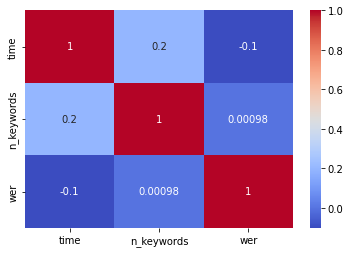
\includegraphics[width=0.6\textwidth]{images/corr_mat.png}
    \caption{Correlation matrix between the \gls{wer}, number of keywords and transcription time.}
    \label{fig: correlation_matrix}
\end{figure}
Figure \ref{fig: transcription_time} displays the transcription time as a function of the number of words. We see that the data is distributed in a quasi-linear fashion. From the slope and intercept coefficients, we have that the transcription time is given by:
\begin{equation}
    \label{eqn: transcription time per number of words}
    y = 0.21 x + 0.41
\end{equation}
which means that there is a ``start time" of 0.41 seconds, then every word takes roughly 0.21 seconds to be transcribed. It has been established that we define near real-time performance as lagging less than 10 seconds, so the number of words that can be transcribed with such a constraint is given by:
\begin{align*}
             & 0.21 x + 0.41 < 10 \\
    \implies &
    0.21 x < 9.59                 \\
    \implies &
    x < \frac{9.59}{0.21}         \\
    \implies &
    x < 45.666\ldots              \\
\end{align*}
Therefore, the maximum number of words that can be transcribed with near real-time performance is 45. Note that this is a raw value and it would probably be wiser to use confidence intervals to ensure that most cases (\textit{e.g.} 90\% or 95\% of cases) fall under the 10 seconds mark.
\begin{figure}
    \centering
    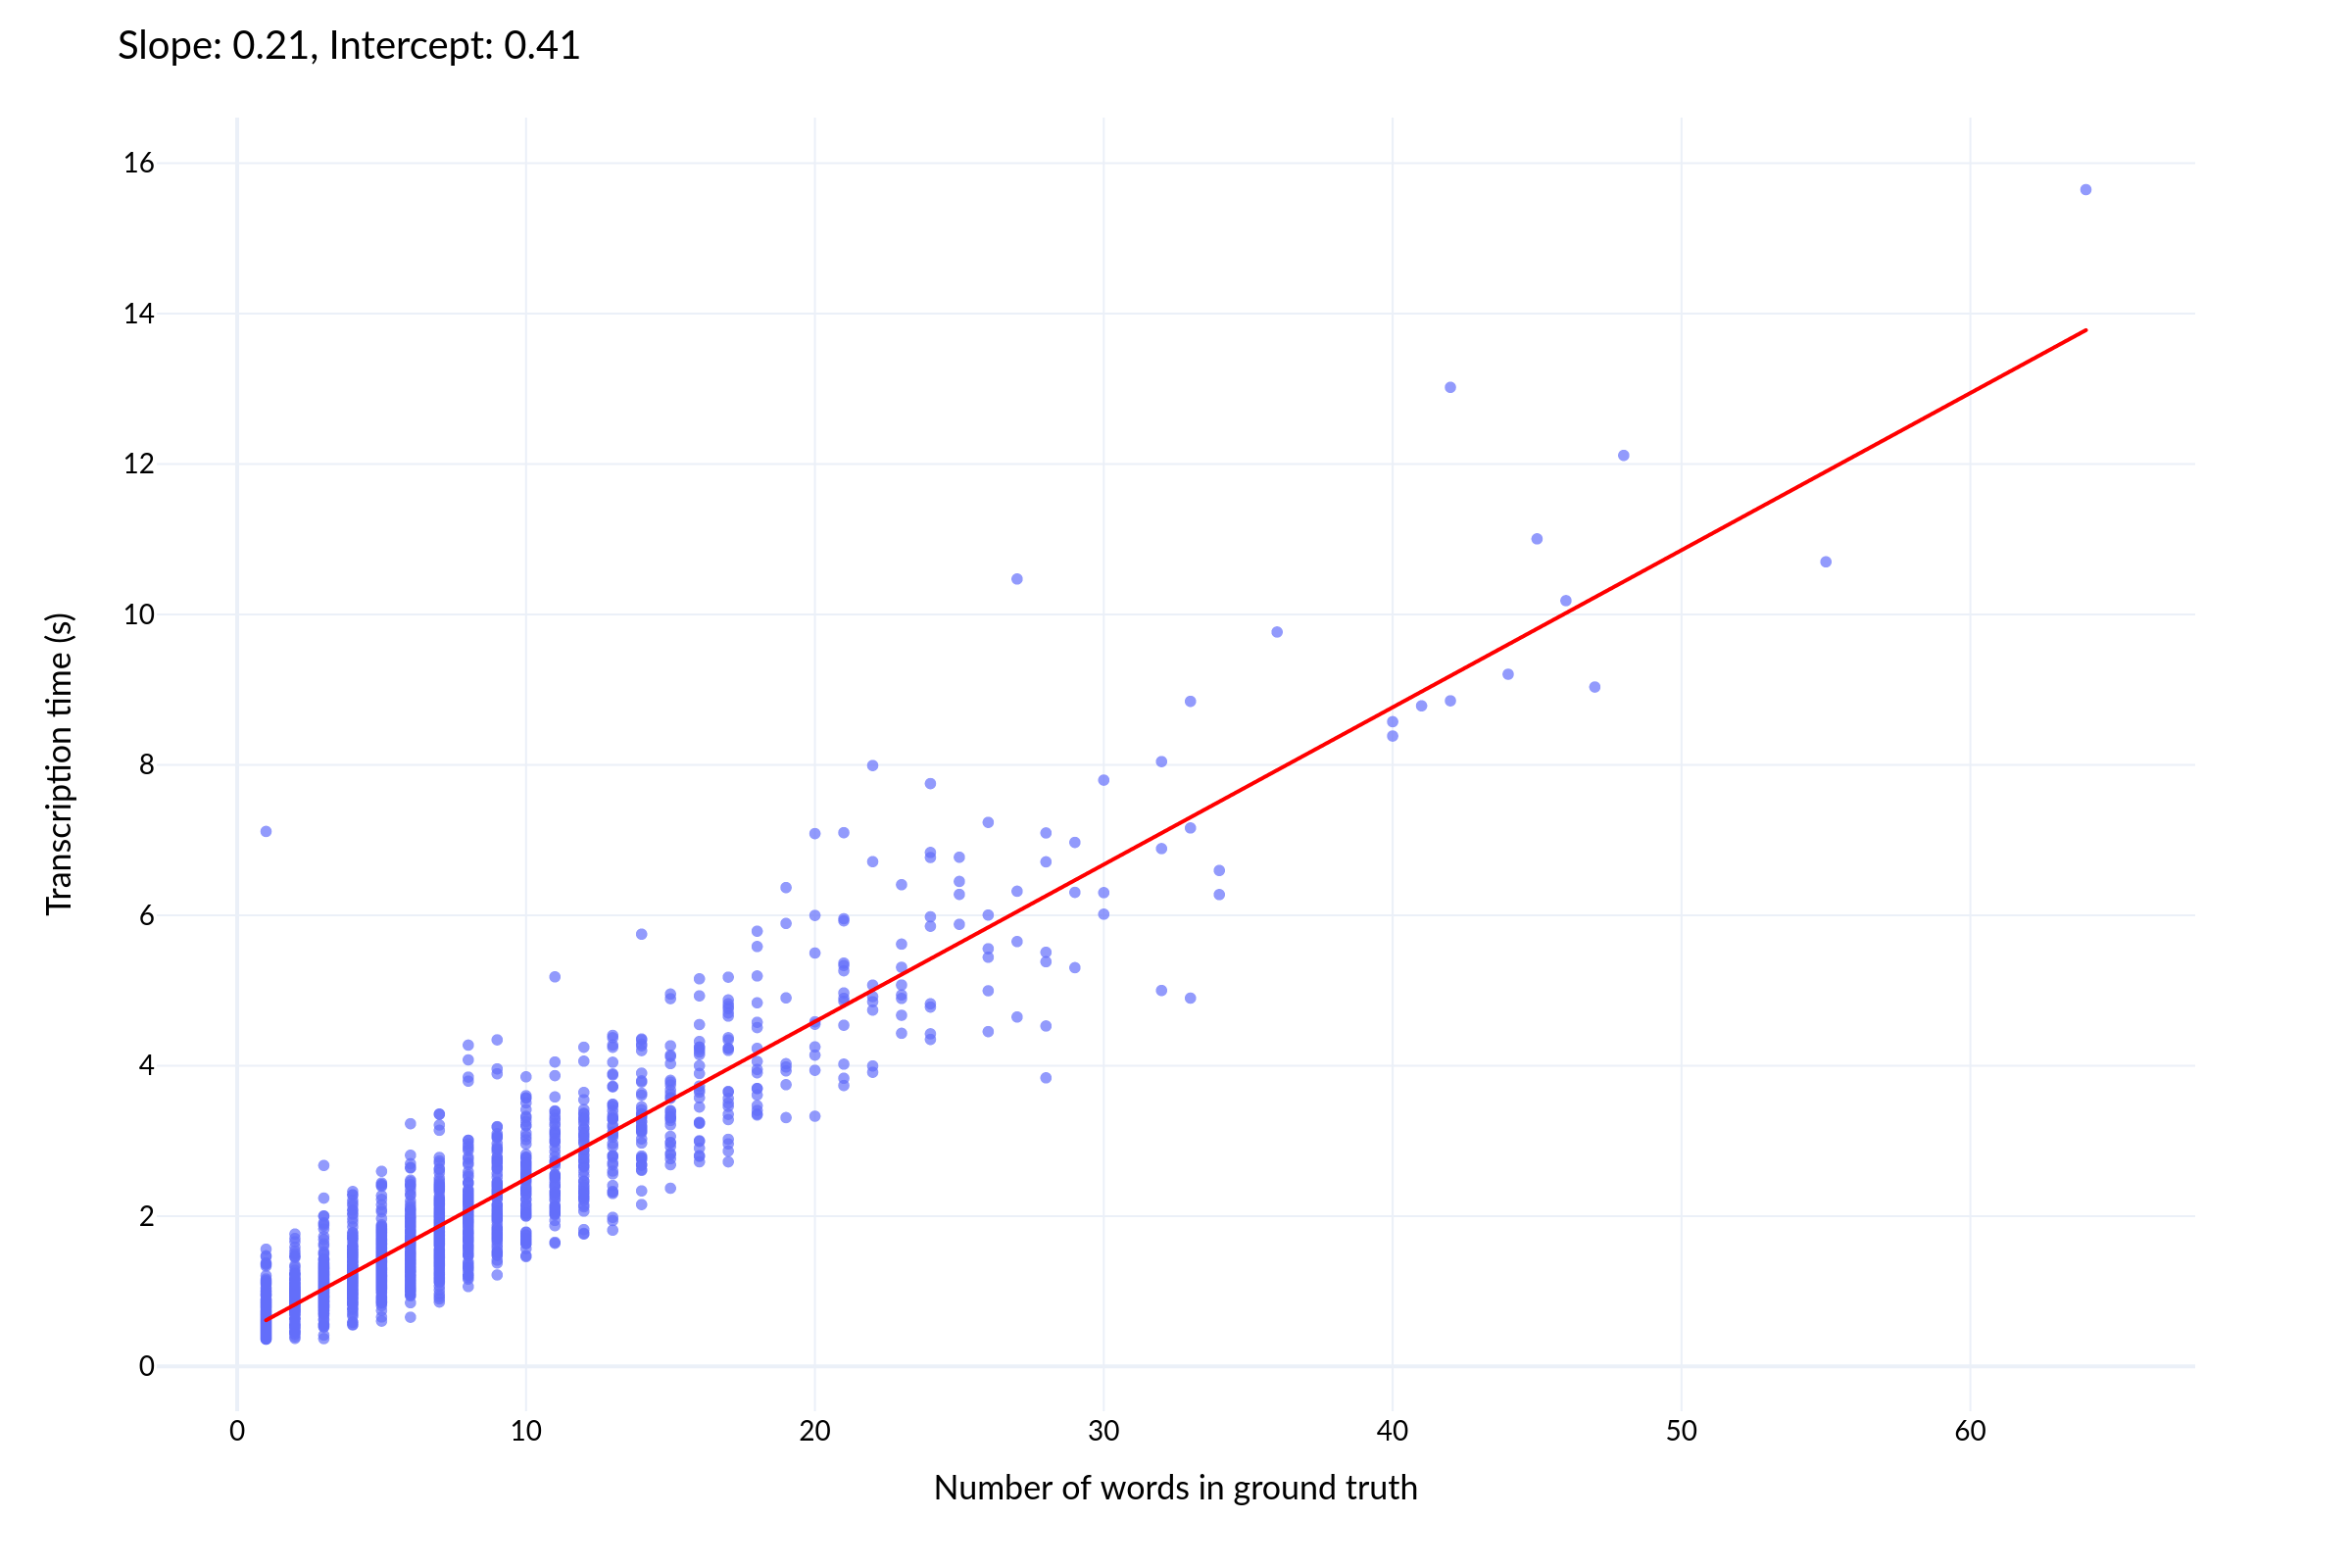
\includegraphics[width=0.9\textwidth]{images/transcription_time.png}
    \caption{Transcription time per number of words}
    \label{fig: transcription_time}
\end{figure}

\section{Conclusion}
Throughout this report, we studied the possibility of deploying a working pre-trained voice recognition engine (\gls{stt}). We saw that for the analysis phase, only some basic rewriting of the audio (WAV) files had to be done. This can certainly be avoided on deployment by directly recording audio files in a format that is compatible with DeepSpeech (for example non-faulty WAV file). This means that DeepSpeech is a free, out-of-the-box solution that can easily be embedded and deployed (for example in a mobile application). \\
Since the ease of use of this solution has been shown, the other major question is the one of performance. We observed that on an average laptop, near real-time performance (lag $<10$s) is reached when the ground truth contains up to 45 words. However, as noted previously, this is a raw value, that could be made more informative by computing a confidence interval around it. Nevertheless, we think that even by considering a confidence interval and using less-capable devices, the fact that oral queries are usually short (less than 15 words, or even less than 10 words) makes this model fast enough to be deployed. \\
Our conclusion is that this model is a good fit for deployment because it is fast, easy to deploy and the correctness of the transcription is pretty high.


\newpage
\appendix
\section{Code structure}
\begin{figure}[H]
    \centering
    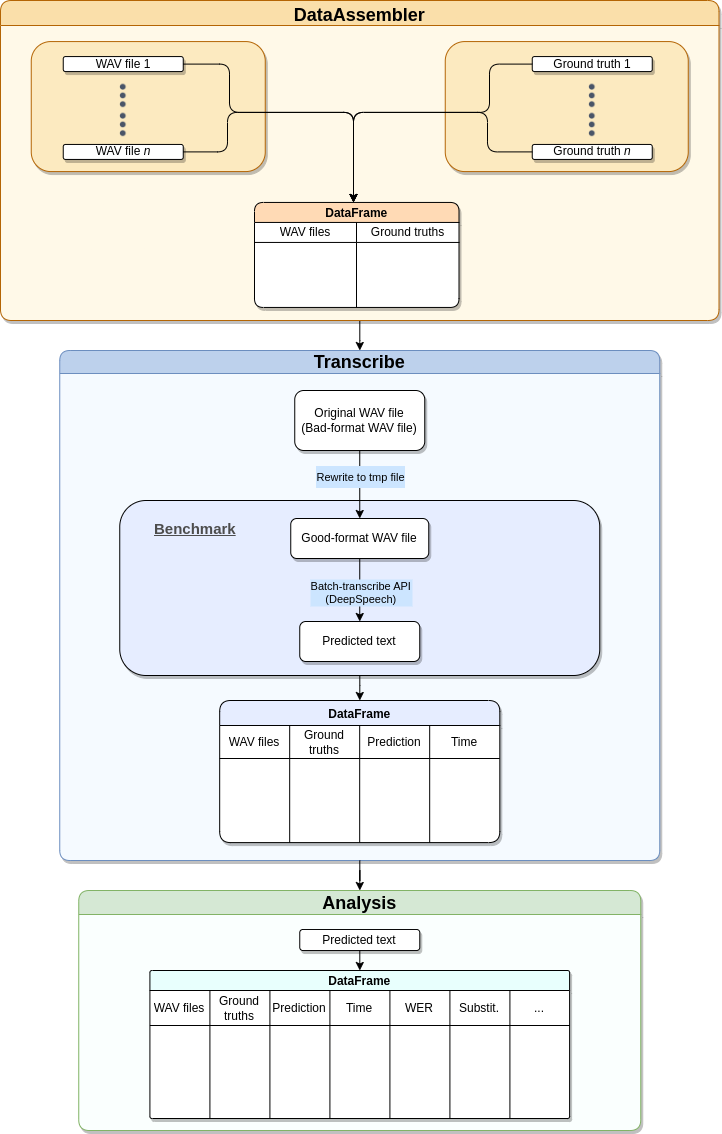
\includegraphics[width=\textwidth, height=0.9\textheight]{images/speech-recognition.drawio.png}
    \caption{Project }
    \label{fig: code structure}
\end{figure}

\section{Specific answers to project presentation questions}

\paragraph{Q1. How complicated is it to deploy a working pre-trained voice recognition engine?}
It is actually very easy to install the model and library from the following websites. Fig \ref{install} shows the example installation commands.

\begin{enumerate}
    \item \textbf{DeepSpeech open source implementation:}\\ https://github.com/mozilla/DeepSpeech
    \item  \textbf{DeepSpeech english pre-trained models:}\\
          https://github.com/mozilla/DeepSpeech/releases/tag/v0.9.3
    \item \textbf{Documentation for installation, usage, and training models:}\\
          https://deepspeech.readthedocs.io/en/r0.9/?badge=latest
\end{enumerate}

\begin{figure}
    \centering
    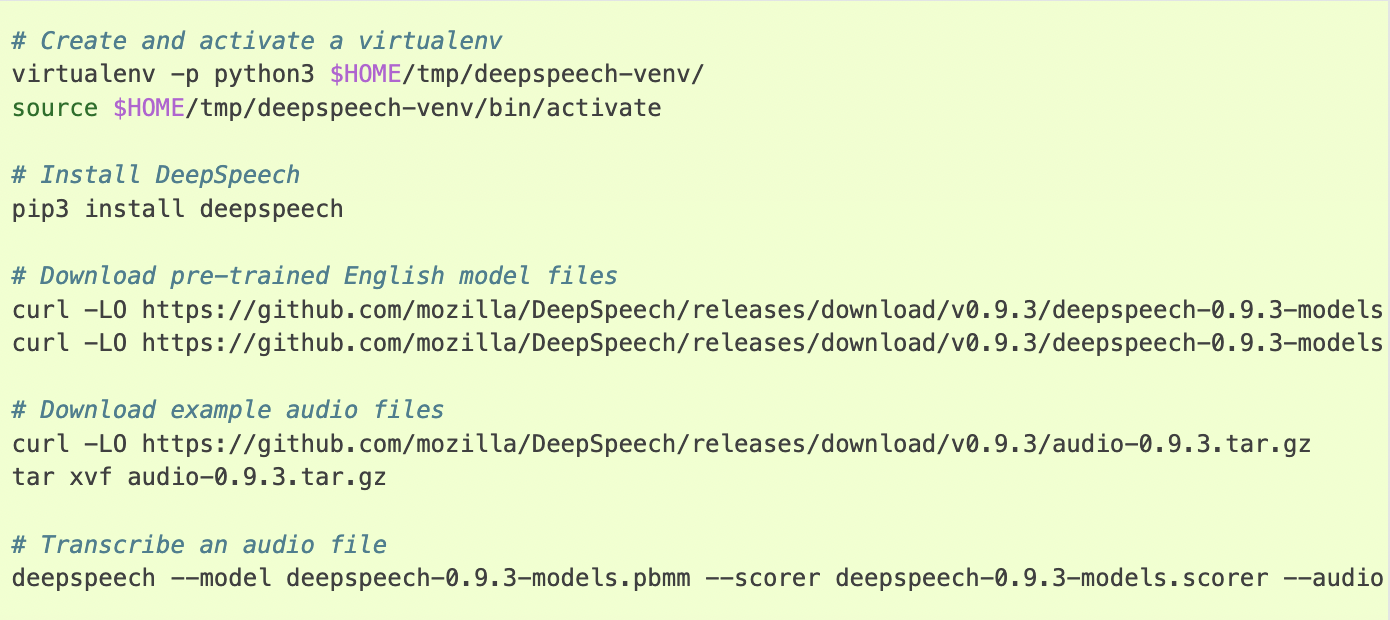
\includegraphics[width=.7\textwidth]{images/installation.png}
    \caption{Some basic command to install DeepSpeech model and library.}
    \label{install}
\end{figure}

The only error that we got was RIFF id error. What this error is and how to handle is explained in Section \ref{riff error}.
This error wouldn't occur on deployment however, because audio files can be directly recorded in the right format.
\paragraph{Q2. Is the engine able to approach near real-time performance? (lag less than 10 seconds)} Yes, for transcriptions of up to 45 words. The general formula is given in equation \eqref{eqn: transcription time per number of words}.

\paragraph{Q3. What is the hardware chosen?} The DeepSpeech model was installed and used on an Asus laptop with the following CPU: Intel(R) Core(TM) i7-4710HQ CPU @ 2.50GHz

\paragraph{Q4. What is the CPU and memory cost of this recognition on the hardware they chose to use?}
We give a benchmark on the device mentioned in Q3. Transcription times on other devices can be inferred from it.

\paragraph{Q5. How good is the recognition?}
Pretty good. Most transcriptions seem decent. See table \ref{result_table} for quantitative results.

\paragraph{Q6. Qualitatively, can you illustrate performance with well-chosen perfect recognitions and illustrate typical mistakes?}
Some words are harder to grab for the model, namely proper nouns like ``Bohemian Rhapsody", whereas more common words are better transcribed.

\paragraph{Q7. Quantitatively, what is the Word Error Rate? How does it compare with state-of-the-art engines on the same dataset?}
The performance is not too far from what the DeepSpeech paper claims on \gls{swb}. Some of the possible reasons for the difference in results are explained in Section \ref{section: results}.


\newpage
\begin{thebibliography}{8}
    \bibitem{deepspeech_paper}
    Hannun, Awni, et al. ``DeepSpeech: Scaling up end-to-end speech recognition." arXiv preprint arXiv:1412.5567 (2014)

    \bibitem{other_model1}
    A. Graves and N. Jaitly. Towards end-to-end speech recognition with recurrent neural networks. In ICML, 2014.

    \bibitem{acoustic_model}
    Swietojanski, Pawel, Arnab Ghoshal, and Steve Renals. ``Hybrid acoustic models for distant and multichannel large vocabulary speech recognition." 2013 IEEE workshop on automatic speech recognition and understanding. IEEE, 2013.

    \bibitem{hmm}
    Juang, Biing Hwang, and Laurence R. Rabiner. ``Hidden Markov models for speech recognition." Technometrics 33.3 (1991): 251-272.

    \bibitem{dl1}
    H. Lee, P. Pham, Y. Largman, and A. Y. Ng. Unsupervised feature learning for audio classification using convolutional deep belief networks. In Advances in Neural Information Processing
    Systems, pages 1096–1104, 2009.

    \bibitem{dl2}
    A. Mohamed, G. Dahl, and G. Hinton. Acoustic modeling using deep belief networks. IEEE
    Transactions on Audio, Speech, and Language Processing, (99), 2011.

    \bibitem{dl3}
    R. Grosse, R. Raina, H. Kwong, and A. Y. Ng. Shift-invariance sparse coding for audio classification. arXiv preprint arXiv:1206.5241, 2012.

    \bibitem{dl4}
    G. Dahl, D. Yu, L. Deng, and A. Acero. Context-dependent pre-trained deep neural networks
    for large vocabulary speech recognition. IEEE Transactions on Audio, Speech, and Language
    Processing, 2011.


    \bibitem{vesely_44}
    K. Vesely, A. Ghoshal, L. Burget, and D. Povey. Sequence-discriminative training of deep
    neural networks. In Interspeech, 2013.

    \bibitem{maas_28}
    A. L. Maas, A. Y. Hannun, C. T. Lengerich, P. Qi, D. Jurafsky, and A. Y. Ng. Increasing
    deep neural network acoustic model size for large vocabulary continuous speech recognition.
    abs/1406.7806, 2014. http://arxiv.org/abs/1406.7806.


    \bibitem{seide_39}
    F. Seide, G. Li, X. Chen, and D. Yu. Feature engineering in context-dependent deep neural
    networks for conversational speech transcription. In ASRU, 2011.

    \bibitem{kingsbury_22}
    B. Kingsbury, T. Sainath, and H. Soltau. Scalable minimum Bayes risk training of deep neural
    network acoustic models using distributed hessian-free optimization. In Interspeech, 2012.

    \bibitem{sainath_36}
    T. N. Sainath, A. rahman Mohamed, B. Kingsbury, and B. Ramabhadran. Deep convolutional
    neural networks for LVCSR. In ICASSP, 2013.

    \bibitem{soltau_40}
    H. Soltau, G. Saon, and T. N. Sainath. Joint training of convolutional and non-convolutional
    neural networks. In ICASSP, 2014.

    \bibitem{data_cite}
    C. Cieri, D. Miller, and K. Walker. The Fisher corpus: a resource for the next generations of
    speech-to-text. In LREC, volume 4, pages 69–71, 2004.

\end{thebibliography}


\end{document}





% \clearpage
% \printnoidxglossaries
